\documentclass[SE,authoryear,toc]{article}
%\input{meta}

% Package imports go here.

\usepackage{graphicx}
\usepackage{caption}
\usepackage{subcaption}

% Local commands go here.
\newcommand{mcat}{m_{\mathrm{cat}}}
\newcommand{mtrue}{m_{\mathrm{true}}}
\newcommand{deltam}{\delta_m}
\newcommand{Deltam}{\Delta\,m}

%If you want glossaries
%\input{aglossary.tex}
%\makeglossaries

\title{Rubin Baseline Calibration Plan}

% Optional subtitle
% \setDocSubtitle{A subtitle}

\author{%
Parker Fagrelius, Eli Rykoff
}

% \setDocRef{SITCOMTN-086}
% \setDocUpstreamLocation{\url{https://github.com/lsst-sitcom/sitcomtn-086}}

\date{\vcsDate}

% Optional: name of the document's curator
% \setDocCurator{The Curator of this Document}

% \setDocAbstract{
% Current baseline plan for the year 1 minimum viable product as delivered for ORR.
% }

% Change history defined here.
% Order: oldest first.
% Fields: VERSION, DATE, DESCRIPTION, OWNER NAME.
% See LPM-51 for version number policy.
% \setDocChangeRecord{
%   \addtohist{1}{YYYY-MM-DD}{Unreleased.}{Parker Fagrelius}
% }


\begin{document}

% Create the title page.
\maketitle
% Frequently for a technote we do not want a title page  uncomment this to remove the title page and changelog.
% use \mkshorttitle to remove the extra pages


\appendix

\section{Introduction}

The basic question of photometric calibration of an astronomical survey is how
to take raw counts output from the camera (in arbitrary Analog-Digital Units
(ADU)) and convert these to calibrated fluxes in nanoJansky (nJy).  In order
for this procedure to yield uniform results across the camera and the sky, it
must take into account variations that are both achromatic (``gray'') and
chromatic, that latter of which depend on the spectral energy distribution (SED) of each
object.  This includes variations in the atmosphere as a function of time and
airmass; spatial variations in the filter and detectors; pixel size variations;
and various sensor effects such as charge transfer ineffeciency (CTI) and the
Brighter Fatter Effect (BFE).

This technote describes the baseline photometric calibration plan for Rubin
Commissioning and the first year of data release production for the LSST
Survey.  This includes plans on performing instrumental signature reduction
(ISR), which is also known as ``detrending''; correct flat-fielding;
background/foreground subtraction; and derivation of a uniform photometric
calibration over the full survey.  It also includes plans for generating
``calibration frames'' such as bias, darks, and various types of flats,
incorporating LEDs, a class 4 tunable laser, and a novel Collimated Beam
Projector (CBP).  We expect that this is not the final calibration plan for the
LSST survey, but rather a first minimal viable product suitable for the first
year of survey observations to meet our required goals for repeatability and
uniformity.  Further improvements are planned to incorporate more effects,
although our plan is to take as much calibration data early on to be able to
reprocess early data with improved algorithms.

The calibration plan in this technote is heavily influenced by the Dark Energy
Survey, which achieved better than $2~\mathrm{mmag}$ uniformity over
$5000\,\mathrm{deg}^2$ in the Southern sky~(Rykoff et al. 2023).  In
particular, we refer the reader to Bernstein et al. 2017 (henceforth B17) and
Burke, Rykoff, et al. 2018 (henceforth BR18).

\section{Requirements}
The requirements on calibration are defined in the Science Requirements Document (LPM-17). The photometric quality and accuracy of the LSST data products is driven by four main components:
\begin{enumerate}
    \item Relative photometry (repeatability)
    \item Stability across the sky (spatial uniformity)
    \item Relative accuracy (color zero-points)
    \item Transfer to physical flux scale (external absolute photometry)
\end{enumerate}

The requirements for photometric calibration accuracy are specified using the following error decomposition (valid in the limit of small errors):
\begin{equation}
    \mcat = mtrue +\sigma+\deltam (x,y,\theta,\alpha,\delta,\mathrm{SED},t)+\Deltam
\end{equation}
where $\mtrue$ is the true magnitude defined by eqs. 4 and 7, $\mcat$ is the cataloged LSST magnitude, $\sigma$ is the random photometric error (including random calibration errors and count extraction errors), and $\Deltam$ is the overall (constant) offset of the internal survey system from a perfect AB system (the six values of $\Deltam} are equal for all the cataloged objects).
Here, $\deltam$ describes the various systematic dependencies of the internal zeropoint error around $\Deltam}, such as position in the field of view (x, y), the normalized system response ($\theta$), position on the sky ($\alpha$,$\delta$),and the source spectral energy distribution(SED).
Note that the average of $\deltam$ over the cataloged area is 0 by construction.

The SRD allocates error specifications for the griz bands, with a 50\% increase expected for u and y bands. These high level allocations are further broken down to three main elements in Observatory System Specifications (LSE-30). These are Instrument Throughput, Atmospheric Transmittance, and Reference Star Catalogs. The full functional error budget can be found in LSST Document-9553.

\begin{table}[|||]
| Design Spec (millimag) | Repeatability | Uniformity | Color Accuracy | External Absolute Photometry |
| Overall Specification | 5 | | 10 | 5 | 10 |
| Instrument Throughput | 3 | 2 | 3 | - |
| Atmospheric Transmittance | 3.5 | 4 | 3 | - |
| Reference Catalog | 2.5 | 9 | 3 | - |

\end{equation}

where $\textrm{m}_{true}$ is the true magnitude defined by eqs. 4 and 7, 
$\textrm{m}_{cat}$ is the cataloged LSST magnitude, $\sigma$ is the random photometric error (including random calibration errors and count extraction errors), and $\Delta$m is the overall (constant) offset of the internal survey system from a perfect AB system (the six values of $\Delta$m are equal for all the cataloged objects). 
Here, $\delta$m describes the various systematic dependencies of the internal zeropoint error around $\Delta$m, such as position in the field of view (x, y), the normalized system response ($\theta$), position on the sky ($\alpha$, $\delta$), and the source spectral energy distribution (SED).
Note that the average of $\delta$m over the cataloged area is 0 by construction.

The SRD allocates error specifications for the griz bands, with a 50\% increase expected for u and y bands. 
These high level allocations are further broken down to three main elements in Observatory System Specifications (LSE-30). 
These are Instrument Throughput, Atmospheric Transmittance, and Reference Star Catalogs. 
The full functional error budget can be found in LSST Document-9553.

\begin{table}
    \begin{tabular}{|c|c|c|c|c|}
        \hline 
        Design Spec (millimag) & Repeatability & Uniformity & Color Accuracy & Abs. Photometry \\
        \hline 
        \hline
        Overall Specification & 5 & 10 & 5 & 10 \\
        \hline
        Instrument Throughput & 3 & 2 & 3 & - \\
        \hline
        Atmospheric Transmittance & 3.5 & 4 & 3 & - \\
        \hline
        Reference Catalog & 2.5 & 9 & 3 & - \\
        \hline
    \end{tabular}

\end{table}

From these functional requirements, requirements are allocated to the Telescope \& Site (LSE-60) and Data Management (LSE-61) systems to ensure that the functional requirements are met. 

\section{Calibration Approach}

This section describes our overall approach to calibration.  There will need to
be other papers detailing aspects.

\subsection{Standard Bandpasses and Standard Sources}

The fundamental goal of photometric calibration is to estimate the surface
brightness of sources across the full sky in a uniform way.  Following B17, we
define $I_*(\theta, \phi, \lambda, t)$ as the surface brightness at an
arbitrary celestial coordinate $(\theta, \phi)$, with wavelength $\lambda$ at a
given time $t$.  For LSST, all survey exposures are 30 seconds, taken in
sequence, so $t$ uniquely identifies a given exposure.  The quantity $I_*$ has
units of power per area per solid angle per wavelength.

There is a different response to photons that are focused by the telescope and
those that are not focused that is very relevant to the way we use flat fields,
as discussed below.  For focused photons, our astrometric calibration can map
photons at position $(x, y)$ to celestial coordinates.  The astrometric
solution also yields the solid angle subtended by each pixel, which we assume
is a nominal value $\Omega_0$ multipled by a relative scaling vector
$\bf{\Omega}$ over the full camera array.  We further note that we must
distinguish between images representing the surface brightness (at a pixel (a
``surface brightness'' image) vs images representing the flux received in a
pixel (a ``fluence image'').  These two images differ by a factor of
$\bf{Omega}$.  We note that aperture fluxes assume fluence images, while
model-fitting fluxes assume surface brightness images.

Following B17, we can model the production of photo-electrons in the detectors
from focused sky photons as the following, for each pixel at $(x, y)$:
%
\begin{equation}
  \mathrm{Rate}(t, x, y) = \Omega_0 \int d\lambda
  \frac{\lambda}{hc}A_{\mathrm{obs}}(\lambda, t, x, y) I_*(\lambda, t, x, y)
  \Omega(\lambda, t, x, y)\\
  = \frac{\Omega_0}{f_1 \times 1\,\mathrm{s}} \int d\lambda I_*(\lambda,
  t, x, y)S_{\mathrm{std}}(\lambda)S_{\mathrm{obs}}(\lambda, t, x,
  y)\Omega(\lambda, t, x, y)
\end{equation}

The value $A_{\mathrm{obs}}$ is the total collecting area times the
transmission of the atmosphere and system, multiplied by the quantum efficiency
of the individual pixel for a given observation.  The constant $1/f_1$ is the
product of the effective area times the photon energy terms.  We define a
dimensionless standard bandpass $S_{\mathrm{std}}(\lambda)$ represents the
spectral response of the system for a typical pixel in typical (standard)
observing conditions.  The function $S_{\mathrm{obs}}(\lambda, t)$ describes
the spatio-temporal deviations from these reference conditions.  As discussed
in BR18, these corrections are minimized with a well-chosen standard passband.
As discussed below, there is an additional challenge with LSSTCam with two
different types of sensors (E2V and ITL), with different characteristic quantum
efficiency as a function of wavelength.  We are faced with a choice of
optimizing our standard bandpass for the center of the focal plane with minimal
corrections there and larger corrections at the edges, or for the full focal
plane with moderate corrections everywhere.

For a point source, the surface brightness incident on the focal plane is
spread by the point spread function (PSF), normalized as:
%
\begin{equation}
  I_*(\lambda, t, x, y) = \frac{f}{\Omega_0}F_*(\lambda)\mathrm{PSF}(\lambda,
  t, x, y),
\end{equation}
%
\begin{equation}
  \Sum_{x,y}\mathrm{PSF}(\lambda, t, x, y)\Omega(\lambda, t, x, y) = 1
\end{equation}
%
\begin{equation}
  \int d_\lambda F_*(\lambda) S_{\mathrm{std}}(\lambda) = 1
\end{equation}
%
Imaging cameras such as LSSTCam can only count photons and not their energy, a
single epoch can only estimate the amplitude $f$ of the stellar flux, and not the
full SED $F_*(\lambda)$.

First, we start with the determination of $f$ for sources which share a
standard reference spectrum $F_{\mathrm{std}}$.  We discuss the case of
different SEDs in the following section.  The goal of photometric
calibration is to ensure we get the same value for $f$ invariant of time or
location on the focal plane.  To properly estimate $f$ from the $\mathrm{Rate}$
image, we define a dimensionless ``reference flat''
%
\begin{equation}
  r_{\mathrm{ref}}(t, x, y) = \int
  d\lambda\,F_{\mathrm{std}}(\lambda)S_{\mathrm{std}}(\lambda)r(\lambda, t, x,
  y)
\end{equation}
%
and construct the fluence image, with units of counts:
%
\begin{equation}
  \mathrm{Fluence}(t, x, y) \equiv T \frac{\mathrm{Rate}(t, x, y)}{r(t, x, y)}
\end{equation}
%
with an exposure time $T$.  Under the assumption that the PSF and area factor
$\Omega$ are independent of wavelength and the width of the PSF (admittedly
naive assumptions; see [refs]), we can esimate the source flux with a simple
sum over pixels in the footprint of the object:
%
\begin{equation}
  \left ( \frac{1\,\mathrm{s}}{T} \right ) \Sum_{x, y} \mathrm{Fluence}(t, x,
  y)\\
  = \frac{f}{f_1}\frac{\int d\lambda
    F_{\mathrm{std}}(\lambda)r_{\mathrm{ref}}(\lambda, t)\mathrm{PSF}(t, x,
    y)\Omega(t, x, y)}{\int d\lambda F_{\mathrm{std}} r_{\mathrm{ref}}
    r(\lambda, t, x, y)}\\
  = \frac{f}{f_1}\Sum_{x, y} \mathrm{PSF}(t, x, y)\Omega(t, x, y)\\
  = \frac{f}{f_1}
\end{equation}
%
Therefore, the reference flat is the quantity we need to get uniform photometry
across the survey.  While this can be roughly approximated by a dome flat
field, as discussed in B17 this must be modified significantly to be suitable
for accurate photometry.

\subsection{Chromatic Corrections}

We need to port over stuff from the FGCM paper on the chromatic corrections,
specifically Section 2.  At least the outline.

At this point, we need to decompose Eqn [above] into the components due to
atmosphere, optics, and sensor.
%
\begin{equation}
  A_b^{\mathrm{obs}} = A\,S^{\mathrm{atm}}(\lambda, t, \mathrm{alt}, \mathrm{az})\,S^{\mathrm{det}}(\lambda,
  x, y)\,S^{\mathrm{opt}}(\lambda, x, y)\,S^{\mathrm{filter}}(\lambda, x, y)
\end{equation}
%
where $A$ is the nominal collecting area, $S_{\mathrm{atm}}(\lambda, t,
\mathrm{alt}, \mathrm{az})$ is the transmission of the atmosphere as a function
of wavelength, time, altitude, and azimuth; $S_{\mathrm{det}}(\lambda,
x, y)$ is the sensor quantum efficiency (QE) as a function of wavelength and
position; $S_{\mathrm(opt)}(\lambda, t, x, y)$ is the transmission of the
mirror and the optics; and $S_{\mathrm{filter}}(\lambda, x, y)$ is the
transmission of the filter as a function of position.

We must assume that these quantities are all constant over a given object
footprint.  We further assume for Year 1 that (a) the filter transmission does
not change with time; (b) the QE and filter transmission is constant over the
scale of a detector; (c) there may be a (c).


\subsection{Foregrounds and Backgrounds}

What to do about foregrounds and backgrounds?

\subsection{Dome Flats and Reference Flux Flats}

This section will describe how we need to know the response to focused light,
and what we need for a smooth background, and what we need to know from the CBP.


\subsection{ISR Operation}

In this section, we describe the instrument signature removal (ISR) for
LSSTCam.  After the photons hit the detector, there are a number of sensor
effects that alter the image as photoelectrons are produced, they are collected
in the detector, clocked and read out, and sent through the amplifier to the
analog-to-digital converter (ADC).  Each of these steps can imprint an effect,
including noise, non-linearities, cross-talk, etc.  Our goal in ISR is to apply
corrections ``in reverse'' to go from the raw camera output (ADU in 16
amplifiers) to a ``post ISR'' image in units of electrons that are equivalent
to the number of photocarriers produced in each pixel incident on the camera.
In this stage we do not correct for quantum efficiency as a function of
wavelength, as that requires knowledge of each individual source SED.

% If necessary we can add in a section about differential non-linearity corrections.

\subsubsection{Overscan Correction}

The first operation we must perform is ``overscan correction'' to remove the
amplifier bias level.  Unfortunately, the bias level in LSSTCam is not
completely stable with time, and thus we require a somewhat complicated
overscan subtraction routine, using both serial overscan (the additional
readout at the end of each row) and parallel overscan (the additional readout
at the end of each column).

First, we perform row-by-row serial overscan correction to remove possible bias
drift and jumps.  [We are investigating a more complex algorithm for some amplifiers
to reduce row-by-row noise.]  We have X overscan pixels per row, and we take
the median of each row, skipping the first two columns, using the afw integer
median sampling algorithm.  [This needs to be written down or referenced
  somewhere].  This introduces approximately XX ADU of noise, which may or may
not be comparable to our read noise, to be calculated.

Next we need to apply parallel overscan subtraction.  One challenge of the
parallel overscan subtraction is that hot columns and saturated stars bleed
into the parallel overscan region, making these columns unusable for
parallel overscan subtraction.  In addition, these bright signals inject a
crosstalk signal into the other crosstalk regions.  Therefore, prior to
parallel overscan subtraction we perform crosstalk correction on just the
parallel overscan region.  As this is done after serial overscan subtraction
(even into the parallel overscan region) this crosstalk correction does not
require extra source detection or background estimation, as in the standard
crosstalk correction described below.  Additionally, we mask the regions with
the saturated parallel overscan and interpolate these.  Finally, we perform
column-by-column parallel overscan correction.  This should be improved.

Not every amplifier on every detector requires the parallel overscan
correction.  Hopefully by the time we get to commissioning we can specify which
amplifiers are problematic, and add a figure here which shows how that works.
Alternatively, new smoother parallel overscan will help a lot everywhere.

\subsubsection{Bias Subtraction}

Next we subtract off any residual common-mode bias structure by subtracting off
a median ``bias'' frame.  The combination of these is described in Section XX.

\subsubsection{CTI Correction}

We must now correct for charge-transfer inefficiency (CTI).  This is due to the
fact that as charge is clocked along the either the serial direction (sCTI) or
parallel direction (pCTI) some small fraction of charge is left behind.  Full
details of our correction algorithm are in [Broughton et al.?].

\subsubsection{Linearity Correction}

We want to ensure that the response of the number of ADU counts that we measure
is completely linear with the incident photons, over a very wide dynamic
range.  We correct for non-linearities using a 10 node spline fit described in
[Astier?].  The generation of the linearity spline fit is described in Section XX.

\subsubsection{Gain Normalization}

From the photon transfer curve (PTC) analysis [ref] we know the gain of each
amplifier.  This might be a model as a function of temperature, TBD.  At this
stage we explicitly normalize each amplifier on each detector to have units of
electrons, with effective gain of 1.

\subsubsection{Variance Plane Creation}

We take the imaging plane and add the read noise per amplifier from the PTC
analysis to create the image variance plane.

\subsubsection{Crosstalk Correction}

We now use crosstalk matrices derived by [ref] to correct the imaging region of
each amplifier.  The crosstalk correction procedure first runs detection to
mask sources and subtract off the background (is this really correct) to
compute the signal that may crosstalk from each source to the other target
amplifiers.  There is no inter-detector crosstalk in LSSTCam.

\subsubsection{Defect Masking and Interpolation}

Next all defects are masked and flagged with a ``BAD`` mask bit.  The defect
finding code is described in [ref] or Section XX.

\subsubsection{Brighter/Fatter Correction}

The Brighter/Fatter effect (BFE) is the effect that as charge accumulates in a
pixel it will distort the local electric field and push further photocharges
away, making brighter objects have a slightly broader PSF.  The correction
algorithm we apply is described in Broughton et al.  This correction is applied
at this stage in the ISR because it is one of the first effects in the signal
chain as the charge is accumulated in the detector.

\subsubsection{Dark Subtraction}

Finally, we subtract the dark frame which is computed from a full dark frame.
The dark rate is quite small, adding only XX electrons per pixel for our
typical 30s exposure time.

\subsection{Applying Flats}

As described above, flat fielding a wide field imager to our precision is
particularly complicated.  We make use of two primary flats generated from
calibration products, the ``background flat'' and the ``reference flux flat''.
The first is used to flatten the \emph{background}, making background
subtraction easier.  The second is used to flatten the \emph{photometry}
without inducing other pixel-level distortions that confuse QE effects with
pixel size effects.



\subsection{Global Calibration}

\section{Flat Field System}


\section{CBP}

Flatfield system consists of four main parts: a calibration screen, an aspheric reflector optic, a tunable laser and a white light system. 

The calibration screen will be illuminated by either the white light system or a tunable laser. The white light system will be used for daily flats, while the tunable laser will be used to create monochromatic flats. Both illumination systems are mounted on the dome and co-rotate with the calibration screen. The output of each is co-located at the center of the calibration screen and can be switched between. In order to project that light onto the screen, and additional optic is mounted on the back of the camera and pancake wrap. This is located precisely 3 meters from the projector. It is critical that the projector is aligned with the reflector to ensure a flat illumination pattern on the calibration screen. 

\subsection{Calibration Screen}
The calibration screen is a large reflective surface that can be aligned with the primary mirror and send diffuse light directly to the telescope and camera. It is large enough to illuminate the whole telescope at one time. The surface itself has a diameter of 10.27 meters and an inner diameter of 3.18 meters. Of this area, the section from a diameter of 4.18 - 9.27 meters is coated with a highly reflective material. The outer and inner rings are coated with a very absorptive material. The screen is built of several small panels, with 16 panels making the outer ring and 8 panels making the inner ring. They are secured to a structure such that they are all flat to 3mm across the whole surface. The panels are coated with Labsphere Permaflect 94\% and 5\% respectively. 

The structure on which the panels are mounted can rotate from 0 to -23 degrees relative to horizontal using an actuator. In this way, it can be tilted so that the optical axis of the telescope aligns with teh optical axis of the screen. There will also be 4 retroreflectors mounted around the screen that can be seen by a laser tracker that is mounted on the telescope so that the screen can be easily aligned with the telescope on a daily basis. 

Requirements for the screen can be found in LTS-523 and drawings can be found in LTS-126.

\subsection{Reflector}
The optic that is used to illuminate the calibration screen in full take the shape of an asphere, which is a radially symmetric optic with a radius of curvature that varies radially. The Rubin Observatory aspheric reflector optic was made from a single piece of aluminum, which was necessary given it's unique shape. The shape of the asphere is given by the following function:
\begin{equation}
Z(s) = \frac{C s^{2}}{1+\sqrt{1-(1+k)\,C^{2}s^{2}}} + A_{4}s^{4} + A_{6}s^{6} + ...
\end{equation}


where Z is the sage of the surface parallel to the optical axis, s is the radial distance from the optical axis, C is the curvature, k is the conic constant, and $A_{n}$ are the aspheric coefficients.
 For this asphere, $C=1/551.4041743$, $k=-3.92683047$, $A_{4}=0$, and $A_{6} = -3.737203\times10^{-18}$.

The shape and reflectivity of the optic were measured in the laboratory. The shape was found to match the function within a micron. The reflectivity and scatter from the optic does change across the optic, varying in reflectance from 78 - 82\% across the optic.

As mentioned above, the reflector is mounted on the back side of the camera and the pancake wrap. It is mounted on its own hexapod, which can be adjusted manually. When installed, it will be carefully aligned with the optical axis of the telescope, using this hexapod, and then secured in place.

The reflector has a cover which can be opened by command using linear actuators. 

\subsection{Tunable Laser}
The tunable laser is an Ekspla NT242 and capable of producing light from 300 - 2600 nm in 1 nm steps (see fig. \ref{fig:laser_power}). It does this by using a combination of a tunable parametric stage using OPO crystals and a sum frequency generation stage. 
Addiitonally, this laser has a spectral cleaning unit, which slightly reduces the output power but increases the spectral purity by removing some of the primary and secondary harmonics using a prism. The laser interfaces to a Fiber Coupling unit, which makes is easy to switch between outputs, two of which focus the light into fibers. 
In this way, we can easily switch between sending the light to the flat field or the Collimated Beam Projector. 

The laser is designed to operate in room temperature air (18-25$^{\circ}$C). 
It will be housed in an aluminum structure mounted to the dome near the calibration screen and sitting below the CBP. 
The laser will be kept within this operating temperature range as much as possible using heaters used in a small area ($<$100W). After use of the laser, heat will be removed from the enclosure using fans until the enclosure is within 2 degrees of the ambient dome environment.
The laser light will be fed into a NA 0.22 optical fiber (Ceramoptic WFNS) and travel $\sim$ 15 m from the laser platform to the CBP and central projector. 

The laser can be operated in continuous mode or burst mode. 
The pulse duration is 3-6 ns, with a repetition rate of 1000 Hz. 
In continuous mode it will continue to send pulses at this rate. 
In burst mode, you can select a number of pulses sent in a ``burst", after which it will not emit until you tell the laser to send another burst.

\begin{figure}[h]
    \centering
    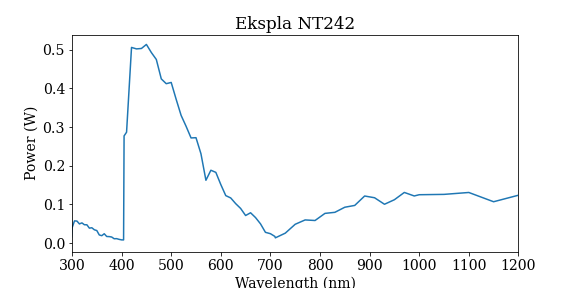
\includegraphics[width=\textwidth]{nt242_output.png}
    \caption{Expected Power output of NT242 Tunable Laser}
    \label{fig:laser_power}
\end{figure}


\subsection{White Light System}
plot of LEDs
Mechanical configuration
Optical model
Model output

\subsection{Projector}

\subsection{Monitoring systems}

We will want to measure precisely how much light from the laser is entering the CBP at a given wavelength so that we determine the exact fraction of that light that is captured by the LSST camera. In order to do that, we need to monitor the luminosity of the laser as it enters the integrating sphere as well as the spectral properties of the light. This data will be recorded for every measurement made with the CBP in such a way that it can be easily linked to the LSST camera image. 

\paragraph{\textbf{Photodiode}}

In order to monitor the exact amount of light injected into the CBP, we use a Hamamatsu S2281 Silicon Photodiode that has been precisely calibrated by NIST. 
This photodiode, which is mounted directly to the integrating sphere, has a sensitive area of 11 mm in diameter. It is read out by a Keithley 6517b electrometer. The electrometer can measure current, charge, resistance and voltage. Our uses of the CBP will likely use the charge and current modes. 

The electrometer can be read out as quickly as every 20 ms. There is a relationship between how long of an exposure you can take and the integration time. At the minimum integration time, you can take an exposure of $\sim$30 seconds. The data is saved in a fits file in the lfa with the elapsed time from the start of the exposure and the value measured. The range can be set to any value from X to Y. 

\paragraph{\textbf{Fiber Spectrograph}}

The spectral response of the injected light will be measured by a pair of fiber-fed spectrographs from Avantes SensLine, one for the blue wavelengths (range) and one for the red (range). These spectrographs will actually be housed in the central projection area in the center of the calibration screen. This is where light from the laser can be projected on the calibration screen. The fibers will be situated such that they will measure some fraction of reflected light within the projector box. When we want to measure the spectral response of the light, we will inject the fiber that runs to the calibration screen, take our measurement, and then send the laser light to the CBP. This assumes that the spectral response will not change from one output to another, which we will have to confirm.

The data from the spectrographs will be saved in a fits file in the lfa that will include the wavelength array and the counts measured by the spectrograph at that spacing.

\section{CBP}
The Rubin CBP was built by DFM Engineering. 
The design is essentially a Schmidt camera used in reverse. 
It includes a primary mirror of 33cm diameter, Schmidt Corrector and a 3-element Flat Field Corrector. 
It produces a beam with an aperture of 24.1 cm and a field of view of 4.1 degrees. 
The focal length of the CBP is 625mm, and with the LSST focal length at 10.1m, the magnification factor is 16. Therefore, a 100$\mu$m pinhole on the CBP would correspond to 1600 $\mu$m, or 160 pixels. 

\begin{table}[h!]
    \centering
    \begin{tabular}{|c|c|}
      \hline
       Aperture   & 24.1 cm \\
      \hline
      Focal Length   & 62.5 cm \\
      \hline
      Field of View & 4.1 degrees \\
      \hline
    \end{tabular}
    \caption{CBP Specifications}
    \label{tab:my_label}
\end{table}

The mount of the CBP allows movement in Azimuth and Elevation, with a swing diameter of 51.8". 
The locations are controlled by a Galil Digital Motor Controller (DMC) that is mounted on the azimuth housing. It controls the motors, reads the encoders, and interfaces to the control computer over ethernet. 
Additionally, the DMC controls the focus of the primary mirror and changes and rotates the masks. 
The azimuth and elevation stages are absolutely encoded with a Renishaw 26-bit on axis encoder. 


\begin{figure}[h]
    \centering
    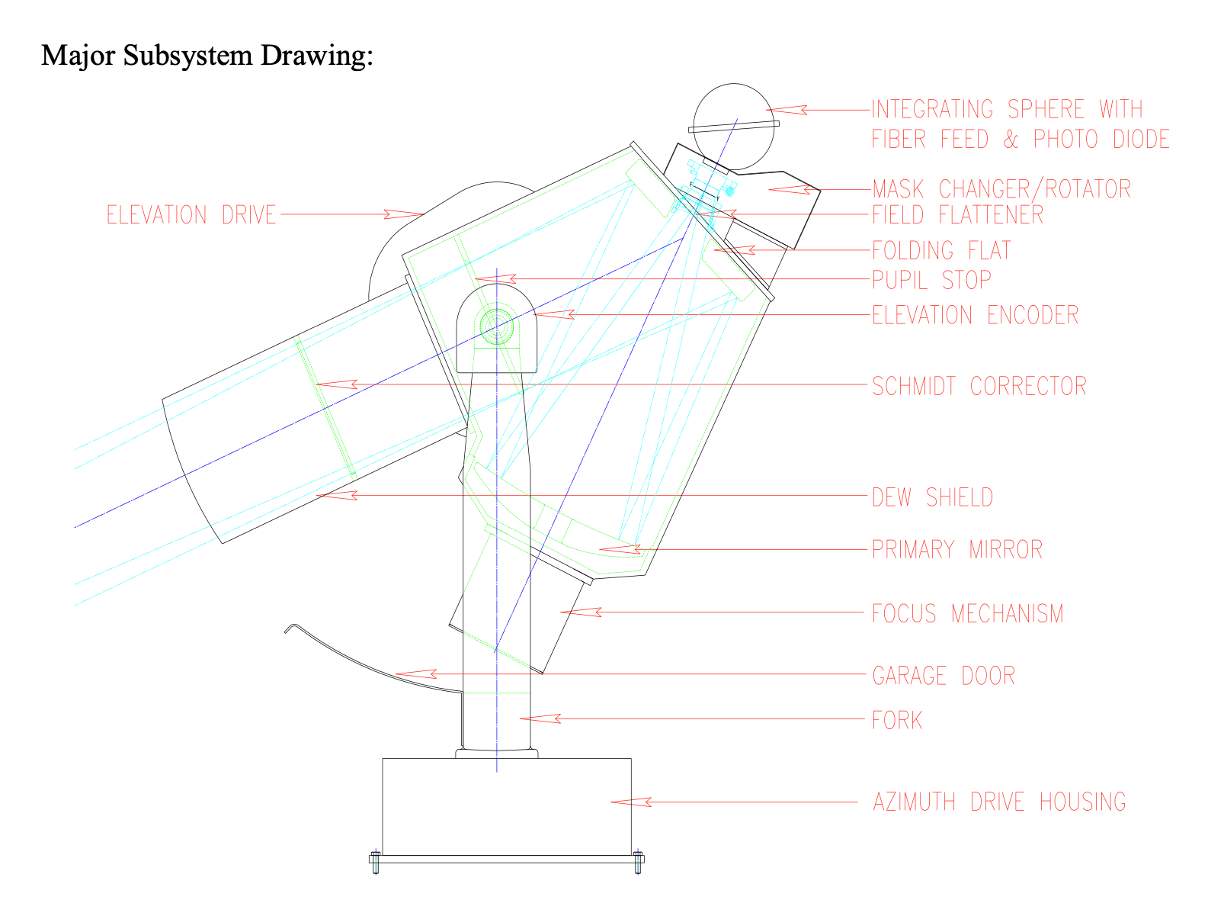
\includegraphics[width=\textwidth]{cbp_drawing.png}
    \caption{CBP Major subsystems}
    \label{fig:laser_power}
\end{figure}

At the focal plane sits the mask stage, which can hold 5 different masks. The masks can be rotated, driven by worm gears such that all masks are rotated on a common shaft by a single motor. The center mask stage is position encoded using a Renishaw absolute rotary encoder. The mask holder can hold masks with a diameter of 50 mm. Each mask will be laser etched into aluminium and are removable/interchangeable. 

The current Integrating Sphere installed on the CBP is a Labsphere 3P-GPS-060-SF. 
This integrating sphere has an interior diameter of 6 in. (152.4mm) and an exit port of 2.5 in. (63.5 mm), coated with spectraflect coating. 
In the exit port a photodiode will be mounted and it will be illuminated by an optical fiber.
The integrating sphere is held to the mask stage with standoffs. 
It sits $\sim 3$ in. from the focal plane/mask. 
Using \url{https://www.labsphere.com/wp-content/uploads/2021/09/Integrating-Sphere-Theory-and-Applications.pdf} as a guide to calculate the intensity of light exiting the integrating sphere by multiplying Ls by the flux incident on the integrating sphere.

\section{AuxTel/LATISS}

\section{Camera EOTest Data}

\section{On-Sky Data}
\subsection{Twilight Flats}
\subsection{Dense Dithered Star Fields}

\section{Plans Post-Year 1}
\subsection{Synethetic SED matched flats}
\subsection{Full CBP dataset}
% Include all the relevant bib files.
% https://lsst-texmf.lsst.io/lsstdoc.html#bibliographies
\section{References} \label{sec:bib}
\renewcommand{\refname}{} % Suppress default Bibliography section
\bibliography{local,lsst,lsst-dm,refs_ads,refs,books}

% Make sure lsst-texmf/bin/generateAcronyms.py is in your path
\appendix
\section{Calibration Products List}


\section{Acronyms} \label{sec:acronyms}
\addtocounter{table}{-1}
\begin{longtable}{p{0.145\textwidth}p{0.8\textwidth}}\hline
\textbf{Acronym} & \textbf{Description}  \\\hline

CBP & Collimated Beam Projector \\\hline
GPS & Global Positioning System \\\hline
ISR & Instrument Signal Removal \\\hline
LATISS & LSST Atmospheric Transmission Imager and Slitless Spectrograph \\\hline
LPM & LSST Project Management (Document Handle) \\\hline
LSE & LSST Systems Engineering (Document Handle) \\\hline
LSST & Legacy Survey of Space and Time (formerly Large Synoptic Survey Telescope) \\\hline
LTS & LSST Telescope and Site  (Document Handle) \\\hline
NIST & National Institute of Standards and Technology (USA) \\\hline
QE & quantum efficiency \\\hline
SE & System Engineering \\\hline
SED & Spectral Energy Distribution \\\hline
SF & Structure Function \\\hline
SRD & LSST Science Requirements; LPM-17 \\\hline
\end{longtable}


\begin{table}[h!]
    \begin{tabular}{|c|c|}
    Quantity & Product Description \\
    \hline \hline
    \textbf{Bias} & (combined) \\
    \hline
    \textbf{Dark} &  (combined) \\
    \hline
    \textbf{CTI} & what are these? \\  
    \hline
    \textbf{PTC} & Linearity + Gain \\
    \hline
    \textbf{C$_{i}$} & Crosstalk Matrix \\
    \hline
     & Defect masks \\
    \hline
    \textbf{BF} & Brighter-fatter kernels \\
    \hline
     & Fringe templates (zy) \\
    \hline
     & Lateral e-field templates \\
    \hline
    \textbf{QE$_{det}$} & Sensor QE \\ 
    \hline
    \textbf{R$_{mirror}$} & Mirror reflectivity (Silver x3) \\
    \hline
    \textbf{T$_{filter}$} & Filter transmission \\
    \hline
     & “White” light flats (ugrizy) \\ 
    \hline
    \textdf{T}(det, $\lambda$) & Transmission \\ 
    \hline
     & Dust flat (?) \\
    \hline
     & Twilight flats (ugrizy; combined) \\
    \hline
     & Sky flat (combined; ugrizy) \\
    \hline
     & Reference Flux Flat \\
    \hline
     & Dense dithered star field + lateral e-field (ugrizy) \\
    \hline
     & Survey observations \\
    \hline
    \end{tabular}
\end{table}

% \section{Acronyms} \label{sec:acronyms}
% \addtocounter{table}{-1}
\begin{longtable}{p{0.145\textwidth}p{0.8\textwidth}}\hline
\textbf{Acronym} & \textbf{Description}  \\\hline

CBP & Collimated Beam Projector \\\hline
GPS & Global Positioning System \\\hline
ISR & Instrument Signal Removal \\\hline
LATISS & LSST Atmospheric Transmission Imager and Slitless Spectrograph \\\hline
LPM & LSST Project Management (Document Handle) \\\hline
LSE & LSST Systems Engineering (Document Handle) \\\hline
LSST & Legacy Survey of Space and Time (formerly Large Synoptic Survey Telescope) \\\hline
LTS & LSST Telescope and Site  (Document Handle) \\\hline
NIST & National Institute of Standards and Technology (USA) \\\hline
QE & quantum efficiency \\\hline
SE & System Engineering \\\hline
SED & Spectral Energy Distribution \\\hline
SF & Structure Function \\\hline
SRD & LSST Science Requirements; LPM-17 \\\hline
\end{longtable}

% If you want glossary uncomment below -- comment out the two lines above
%\printglossaries





\end{document}
